\mcchap{Design e sviluppo della soluzione}{cap:designSviluppo}
\setlength{\parskip}{1em}

\section{Tecnologie utilizzate}

In questo capitolo verranno elencate alcune delle tecnologie utilizzate per lo sviluppo del progetto.

\subsection{Python}
Python è un famoso linguaggio di programmazione ad alto livello, molto utilizzato nel campo \emph{data science}.
Python dispone di librerie e funzioni matematiche integrate, che semplificano il calcolo dei problemi matematici e l'esecuzione dell'analisi dei dati.
Lo sviluppo del progetto è stato svolto interamente in linguaggio Python 3.


\subsection{Plotly}

Plotly è una piattaforma di visualizzazione dati open source dell’omonima azienda che supporta anche grafici interattivi.
Plotly supporta la rappresentazione di svariate tipologie di grafici.
I linguaggi supportati sono Python, R, e Javascript.
\begin{figure}[htp]
    \centering
    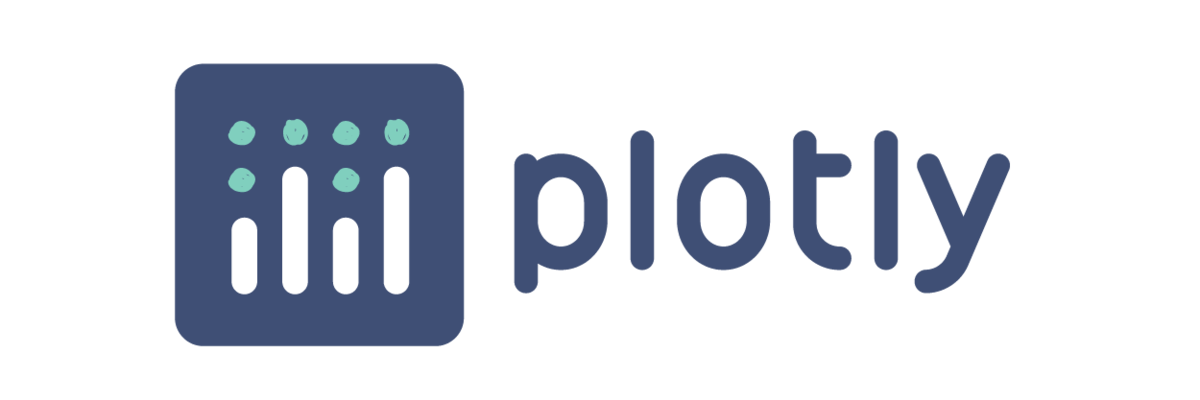
\includegraphics[width=3cm]{plotly_logo}
    %\caption{Logo di Plotly}
\end{figure}

\subsection{Pandas}
Pandas è una libreria Python per analisi e la manipolazione di dati.
Pandas utilizza una struttura dati chiamata DataFrame, si tratta di una struttura dati bi-dimensionale, a dimensione variabile e può contenere potenzialmente dati eterogenei.

\subsection{Dash}
La dashboard è stata realizzata utilizzando Dash, un framework Python ideato per costruzione di applicazioni web di analytics.
\noindent Dash si appoggia a Flask, Plotly.sj e react.js. Dash ideale per la costruzione di applicazioni di visualizzazione dati con elevata personalizzazione in puro Python. E’ particolarmente indicato per chiunque lavori con i dati in Python.

\noindent Attraverso alcuni semplici pattern, Dash astrae via tutte le tecnologie e i protocolli necessari che sono richiesti per costruire e interagire con applicazione basate su web.

\subsection{Docker}
Docker è un progetto open source che automatizza il deployment di un'applicazione.
Docker basa il suo funzionamento su dei container, un contenitore standardizzato che contiene software e le sue relative dipendenze.
E' stato scelto Docker in quanto rende ogni dashboard isolata dalle altre e pertanto semplifica il processo di aggiornamento.


\begin{figure}[htp]
    \centering
    
\includegraphics[width=3cm]{docker_logo}
    %\caption{Logo di Docker}
\end{figure}

\section{Lo sviluppo}

\subsection{Fonte dei dati}
Il Dipartimento della Protezione Civile italiana ha allestito un repository \emph{Github} dove ogni giorno vengono caricati i nuovi dati relativi alla pandemia.

\begin{figure}[htp]
    \centering
    
\includegraphics[width=5cm]{logo_dpc}
    \caption{Logo del Dipartimento della Protezione Civile}
\end{figure}

\subsection{Diagramma di attività}
Un diagramma di attività UML è un diagramma di flusso che rappresenta il flusso del programma da un'attività all'altra,
da un punto iniziale (punto nero pieno) a un punto finale.

\begin{figure}[htp]
    \centering
    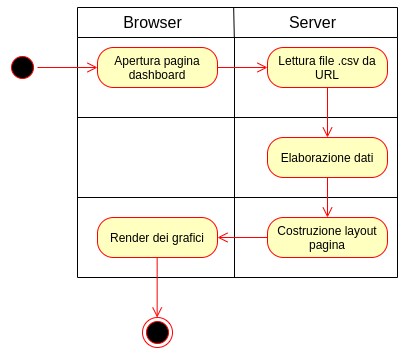
\includegraphics[width=7cm]{activity}
\end{figure}

\subsection{Organizzazione file}

\subsubsection{Italia}

\dirtree{%
.1 italy.
.2 assets.
.3 bootstrap.min.css.
.2 dash\_italy.py.
}

\subsubsection{Lombardia}

\dirtree{%
.1 lombardia.
.2 assets.
.3 bootstrap.min.css.
.2 dash\_lombardia.py.
}

\subsubsection{Regioni}

\dirtree{%
.1 lombardia.
.2 assets.
.3 bootstrap.min.css.
.3 img.
.4 Abruzzo.png.
.4 Basilicata.png.
.4 Calabria.png.
.4 ....
.2 dash\_regioni.py.
}